
\section{Ankle Foot Orthosis}
\label{sec:ankle}
The work done in this section was in collaboration with Nathaniel Michaels. I was the lead designer and gave feedback for the mechanical and electrical design. I also designed and helped run the experiments for the validation of the systems. 

The ankle-foot orthosis (AFO) of LARRE comprises two components, a passive ankle joint to keep the foot straight and a sensor to sense the ground force reactions. The design process of the AFO is discussed in more detail here \cite{Michaels2020}.  A rendering of the AFO mechanism is shown in \autoref{fig:AFO Mechanism Full} and \autoref{fig:Outer Ankle Box fig}. The AFO is designed to fit over the shoe to allow the operator to easily donn and doff the exoskeleton, uses a passive spring to balance the foot's mass and prevent foot drop while still allowing flexion, and the sensing sole detects the phases of the gait cycle. 

\begin{figure}[h!]
    \centering
    \begin{subfigure}[b]{0.45\textwidth}
        \centering
        \captionsetup{justification=centering}
        \centerline{
        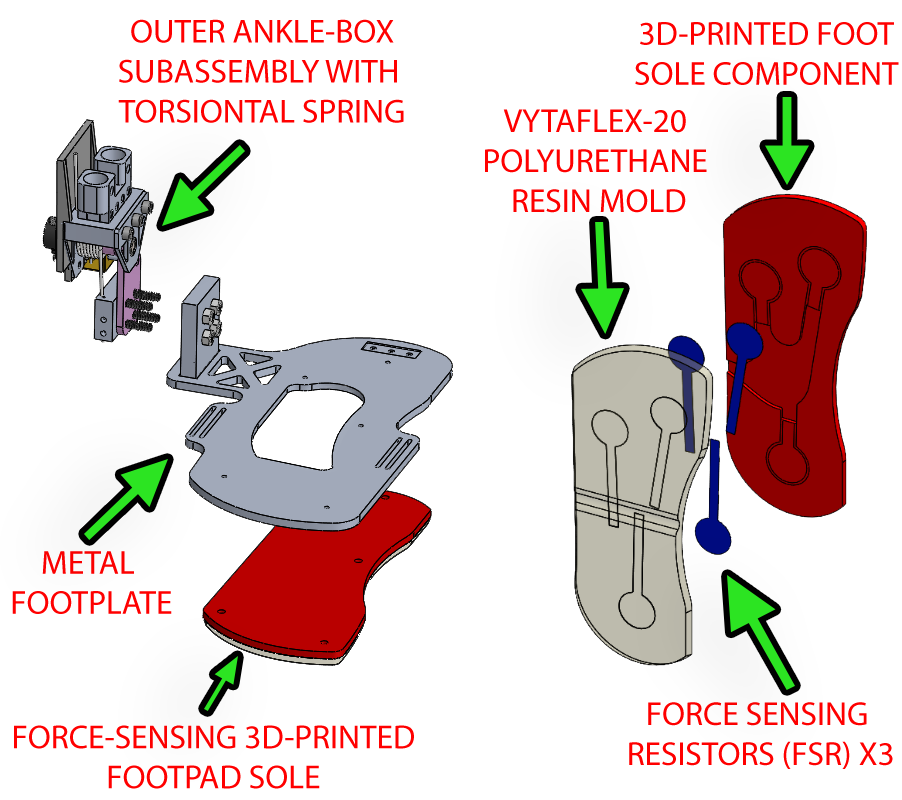
\includegraphics[scale=0.2]{images/mech_design/AFO_Exploded_AND_Force_Sole_WITH_Labels2.png}}
        \caption{AFO Mechanism. There are three parts to the system; the outer ankle box, the sensing sole, and the the metal foot plate}
        \label{fig:AFO Mechanism Full}
    \end{subfigure}
    %
    \begin{subfigure}[b]{.45\textwidth}
        \centering
        \captionsetup{justification=centering}
        \centerline{
        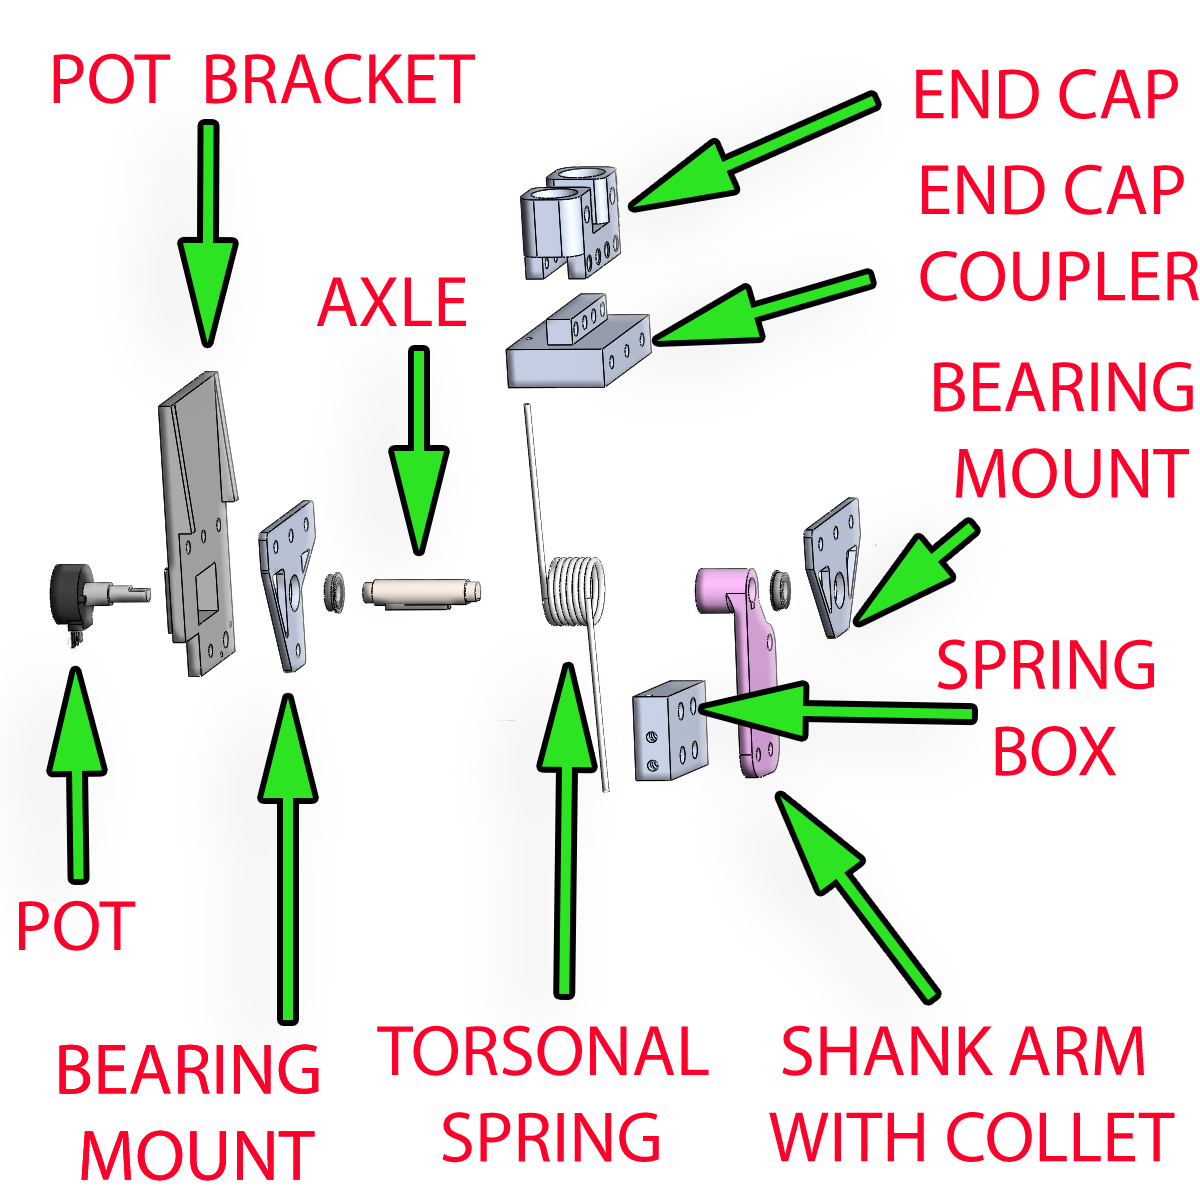
\includegraphics[scale=0.15]{images/mech_design/Outer_Ankle_Box_Exploded_WITH_Labels2.png}}
        \caption{Outer Ankle Box Exploded View. This system transfers the body load from the legs to the floor. The spring }
        \label{fig:Outer Ankle Box fig}
    \end{subfigure}%
    \caption{AFO Sub-Assemblies}
    \label{fig:AFO Sub-Assemblies}
\end{figure}


The sensing sole has Ohmite FSR03C3 Force Sensing Resistors (FSRs) \footnote{https://www.ohmite.com/catalog/fsr-series/FSR03CE} embedded into the toe and heel areas of the sole. FSRs are flat flexible resistors that change their electrical resistance based on the applied force \cite{yaniger1991force} and convert the force to an electrical signal by measuring the sensor's variation of conductivity. The small flexible forum factor force-sensing makes them ideal sensors for wearable devices \cite{giovanelli2016force}.    

FSRs embedded into the sole of an AFO can measure the gait phases. Patar \textit{et. al} two embedded FSRs into their AFO to measure the transition pressure points in the foot during the gait cycle\cite{ab2014system}. In their model, a single FSR was placed on the foot's heel and ball, respectively.  

\autoref{fig:Foot-Force Mapping} shows the sensors' locations relative to the pressure points. The FSRs are encased in a Urethane risen. The risen distributes the ground forces onto the sole and protects the sensors from being damaged. The resin has properties similar to shoes' soles, with a shore hardness of 20 and a non-stick surface \footnote{Vytaflex20Website}. Both Vytaflex-20 \footnote{https://www.smooth-on.com/products/vytaflex-20/} and Vytaflex-30 \footnote{https://www.smooth-on.com/products/vytaflex-30/} were tested as possible options. Once the system was cured, the Vytaflex-30 material had a sticky surface texture. It was not suitable since contact with the ground and dirt and debris would stick to the surface. The Vytaflex-20 material was cured with a surface and was much less sticky, making it better than the Vytaflex-30 material for encasing the sole sensors. 

The Vicon motion capture system and the AMTI force plates were used to measure the center of pressure of the AFO.  The measurement was used to detect the individual reading of the FSR and to validate the AFO's CoP. Each of the FSR's was treated as an on-off switch. If the pressure detected was above a threshold, it was treated as "on," below the threshold as "off."  Several different versions of the AFO were tested; the final version of the sensors readings and filtering is shown in \autoref{fig:FSRBinarized}. As shown, the filtering removes the noise from the sensor reading. \autoref{tab:statetable} shows a state table to detect the different states of the AFO. 

\begin{figure}[h!]
    \centering
    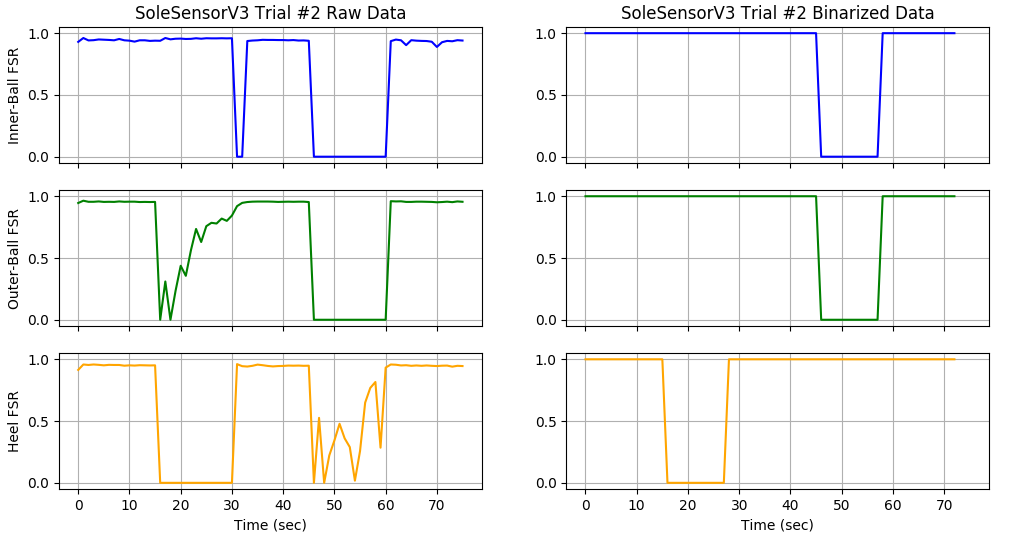
\includegraphics[scale=0.45]{images/mech_design/SoleSensorV3T2_Raw_v_Binarized.png}
    \caption[Measurement of raw FSR]{Measurement of raw FSR activation and filtering \cite{Michaels2020}}
    \label{fig:FSRBinarized}
\end{figure}


\begin{table}[h!]
    \centering
    \begin{tabular}{|c|c|c|c|}
    \hline
    FSR1 - Inner Ball & FSR2 - Outer Ball & FSR3 - Heel & Position-State \\[0.5ex]
    \hline\hline
    0 & 0 & 0 & Foot not on ground \\
    \hline
    0 & 0 & 1 & Heel-Down \\
    \hline
    0 & 1 & 0 & Transition or Error \\
    \hline
    0 & 1 & 1 & Leaning Outward \\
    \hline
    1 & 0 & 0 & Transition or Error \\
    \hline
    1 & 0 & 1 & Leaning Inward \\
    \hline
    1 & 1 & 0 & Toe-Down \\
    \hline
    1 & 1 & 1 & Flat-Foot \\
    \hline
    \end{tabular}
    \caption[AFO State Table]{AFO Position State-Table with FSRs as bits \cite{Michaels2020}}
    \label{tab:statetable}
\end{table}



\begin{figure}[h!]
    \centering
    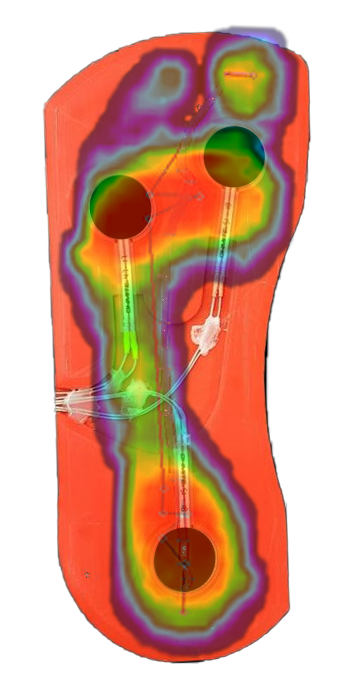
\includegraphics[scale=0.25, angle =-90 , frame]{images/mech_design/sole.png}
    \caption[Pressure Map of Foot]{Overlay of Pressure Map with current Foot Sensor design}
    \label{fig:Foot-Force Mapping}
\end{figure}

Finite element analysis (FEA) was used to validate that the AFO could withstand the applied forces \cite{akin2010finite}. The FEA analysis was conducted using SolidWorks \footnote{https://www.solidworks.com/} FEA tools; this allowed for each of the individual components to be tested and validated before being manufactured. The testing showed that components under the assumed loads, the Von Mises \cite{shigley} stress, did not exceed the materials' yield strength and would not break.

\begin{equation}
\large
    \{x,y\}_{cop} = \sum_{i}^{N} \{x,y\}_i F_i
    \label{eq:FSRCoP}
\end{equation}

The Center of Pressure (CoP) of the AFO is measured by using \autoref{eq:FSRCoP}, where $\{x,y\}$ is the location of the FSR and $F$ is the force of the FSR. The location of FSRs is shown in \autoref{fig:AFOmocap}. The CoP was validated using the mocap and force plates. The force was measured using the force plate, which provides the force along each axis, and the mocap markers located the force vectors in space. The mocap+forceplates were used to dead reckon the FSR sensors. 




 \begin{figure}[h]
    \ContinuedFloat
           \captionsetup{justification=centering}
           \centerline{ 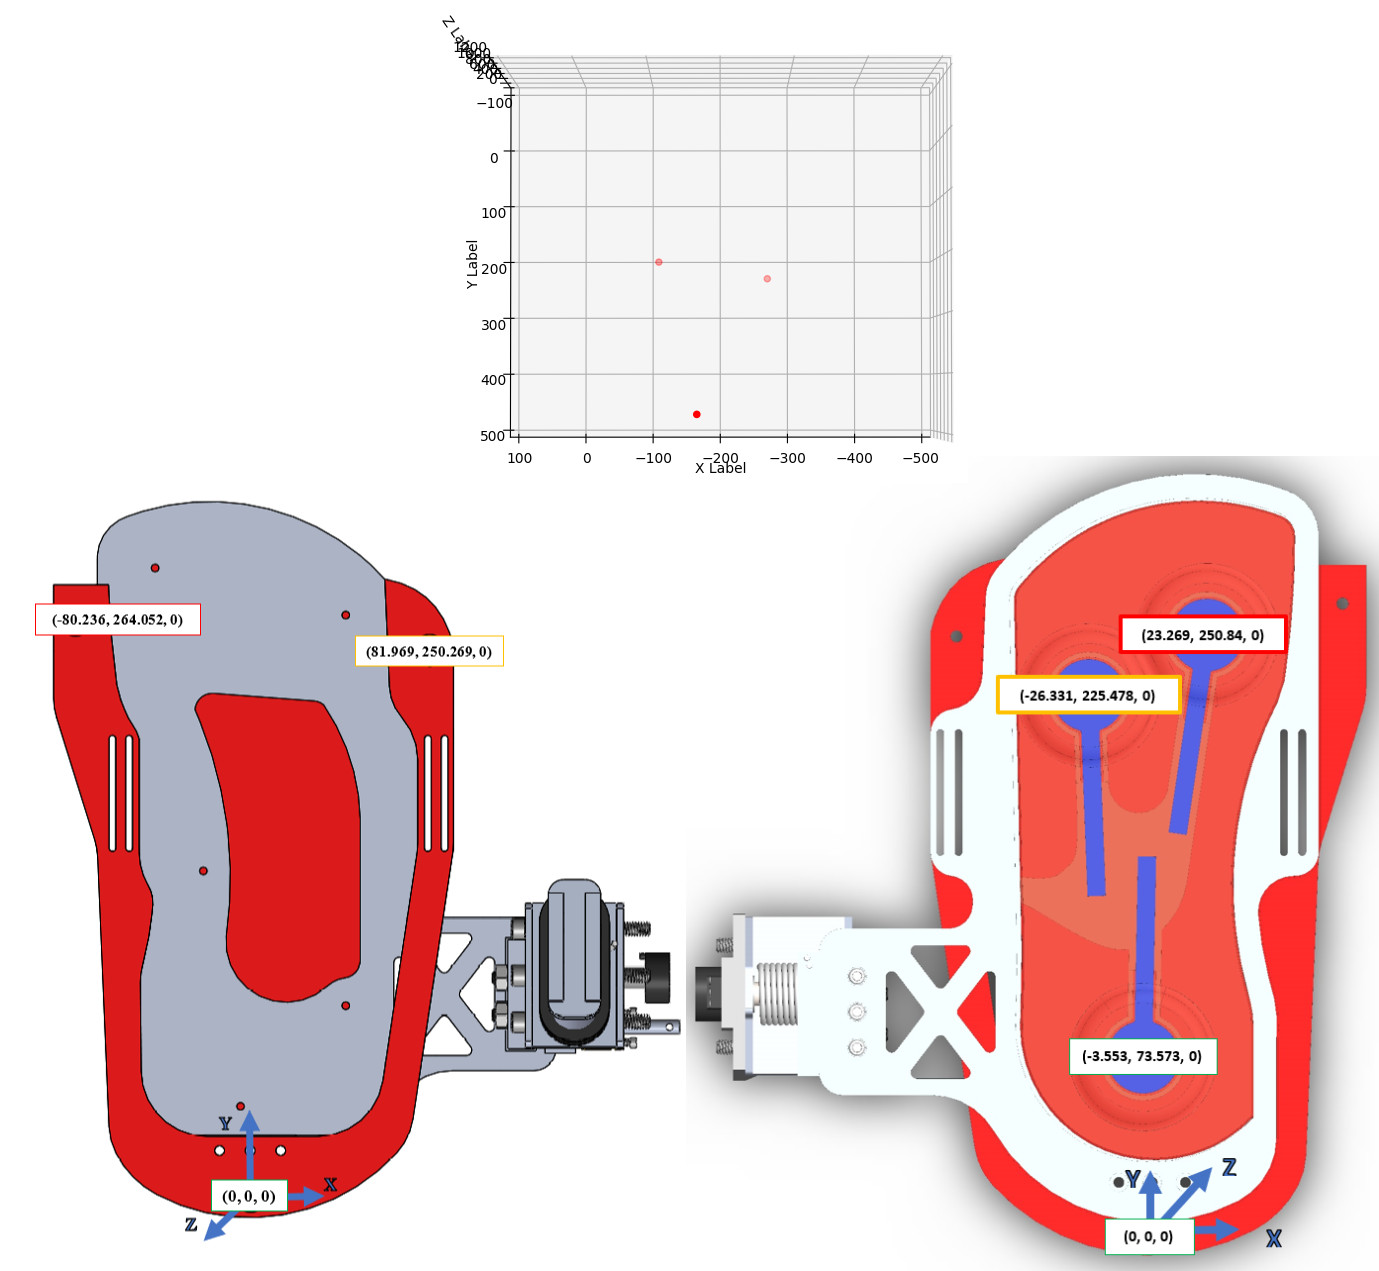
\includegraphics[scale=0.22]{images/mech_design/Mocap_Layout_2.png}}
            \caption[AFO Mocap Markers]{Location of mocap markers and FSRs on the AFO \cite{Michaels2020}}
            \label{fig:AFOmocap}
    \end{figure}


The results of the CoP measurement are summarized in \autoref{fig:3DFSRCoP} and \autoref{fig:FSRCoPAFO} . The shape created by the AFO point shows major distortions across the $x$ axis compared to the force plate. The $z$ axis can be ignored since it is perpendicular to the page and has no significant meaning. The major axis of interest is the $y$ axis that goes along the foot's cardinal longitudinal axis. These FSRs can track the CoP measured by the force plates. 


\begin{figure}[h!]
    \centering
    \begin{subfigure}{0.5\linewidth}
        \captionsetup{justification=centering}
        \centerline{ 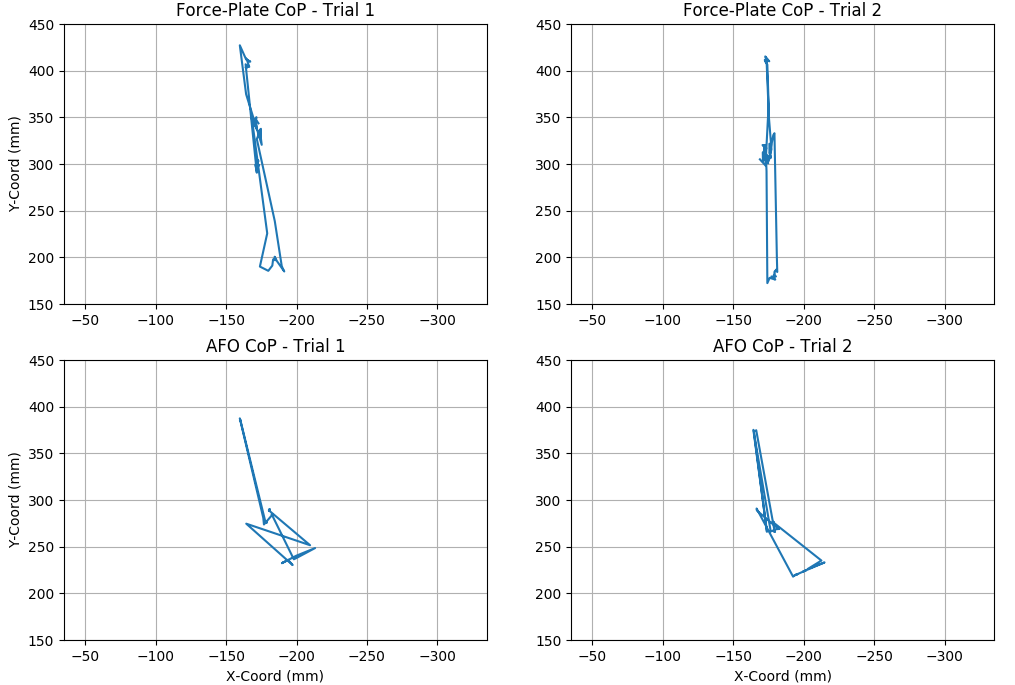
\includegraphics[scale=0.35]{images/mech_design/SoleSensorV3_CoPComparison_2D_XYplane.png}}
        \caption[CoP comparison]{The CoP comparison results between the calculated AFO CoP point and the Force-Plate CoP point within the world frame, across both trials.}
        \label{fig:3DFSRCoP}
    \end{subfigure}%
    \vspace{1cm}
    \begin{subfigure}{.5\linewidth}
        \captionsetup{justification=centering}
        \centerline{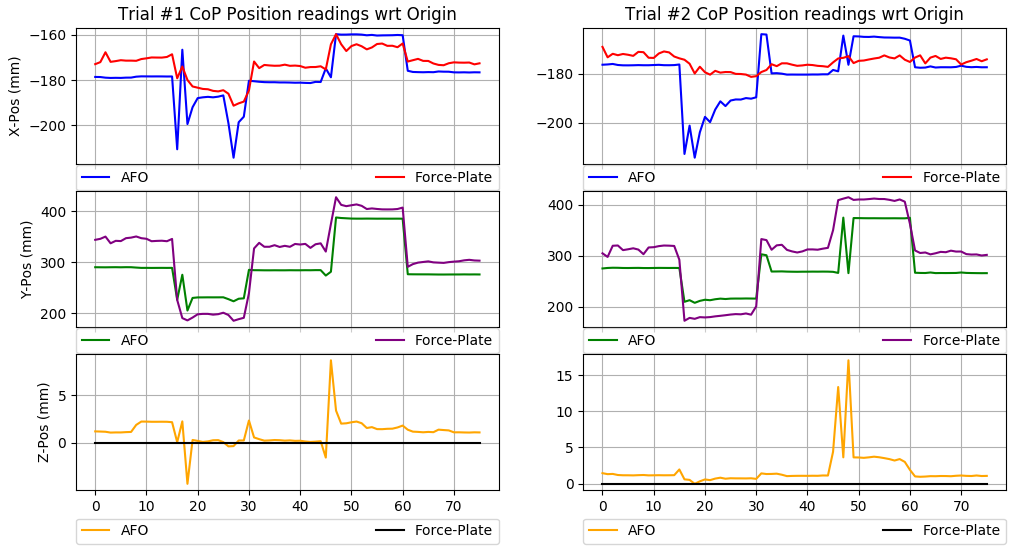
\includegraphics[scale=0.35]{images/mech_design/SoleSensorV3_CoPComparison_BothTrials.png}}
        \caption[CoP Point Trail ]{CoP Point trail created by both the Force-Plates and AFO across both trials. }
        \label{fig:FSRCoPAFO}
    \end{subfigure}%
    \caption[Center of Pressure of the AFO]{Center of pressure of the AFO measured using the FSRs compared to the forceplate measurement \cite{Michaels2020}}
    \label{fig:CoPAFO}
\end{figure}


This device combined passive-dorsiflexion control methods and sensory feedback systems into a single AFO device for LARRE. This device acts as a fully-functional DAFO device capable of controlling foot-drop using a passive torsional-spring system. The devices provide real-time feedback for balance control and force distribution.  Using three FSRs instead of two makes it possible to determine the CoP point within the support polygon they form.  This information can be used by the main controller onboard the LARRE to help the system maintain its balance.

